\section{Lösungsidee}
Um möglichst effizient Kreismittelpunkte zu bestimmen, mache ich mir zunächst folgende Eigenschaft von Kreisen zunutze: Am Mittelpunkt eines Kreises ist der Abstand (Radius) zu der äußeren Umrandung des Kreises in jede Richtung gleich.

In einem Bild lassen sich solche Punkte finden, indem man von jedem schwarzen Bildpunkt misst, wie weit man sich auf dem Bild in vertikale wie horizontale Richtung "`bewegen"' kann, ohne auf ein weißes Feld zu stoßen. Wenn dieser Abstand nach rechts, links, oben und unten gleich groß ist, genügt der Punkt der erstgenannten Eigenschaft von Kreisen. 

Von einem Vergleich des Abstandes in andere Richtungen (wie z.B. in diagonale Richtung) sollte man bei einem Bild aus Pixeln absehen, da bei der Speicherung eines Kreises als Bitmap aus quadratischen Pixeln diagonale Messungen oder gar Messungen unter beliebigem Winkel ungenaue Ergebnisse liefern. Zwar sind solche Messungen prinzipiell möglich, liefern aber anders als rein vertikale oder horizontale Messungen kein ganzzahligen Ergebnisse, da eine Pixeldiagonale \(\sqrt{2}\) Pixelseiten lang ist.\footnote{: \(|\vectwo{1}{1}| = \sqrt{2}\)}

\begin{figure}[!ht]
	\centering	
	\includegraphics[width=0.8\textwidth]{durchmesservergleich}
	\caption{Versch. Formen mit eingezeichnetem Mittelpunkt (erstes Kriterium)}
\end{figure}

Da diese Eigenschaft jedoch auch auf Punkte in Quadraten und anderen unregelmäßigen Formen zutrifft (s. Grafik), muss für eine zuverlässige Erkennung eine zweite Eigenschaft von Kreisen genutzt werden: Bei bekanntem Durchmesser kann die Fläche eines Kreises mit der Kreisformel\footnote{: \(\frac{\pi d^2}{4}\)} bestimmt werden. Diese Soll-Fläche kann mit der tatsächlichen Fläche verglichen werden. Sollte das Delta zwischen diesen beiden Flächengrößen nahe 0 sein, handelt es sich mit sehr großer Wahrscheinlichkeit um einen Kreismittelpunkt.

Daher nehme ich an, dass jeder Punkt, auf den beide Bedingungen zustimmen, ein Kreismittelpunkt ist. Allerdings gibt es aufgrund von Kompressionsartefakten o.ä. manchmal mehrere Punkte, auf die die Bedingungen zutreffen. Damit der Mittelpunkt eindeutig festgestellt wird, vergebe ich bei der Flood-Fill ID's für jede Zusammenhangskomponente. Daher kann ich für Pixel, für die schon eine ID vergeben wurde, die Suche abbrechen. Schließlich wurde entweder schon ein Mittelpunkt gefunden oder es hat sich herausgestellt, dass es sich nicht um einen Kreis handelt.

\begin{wrapfigure}{r}{0.35\textwidth}
  \centering
  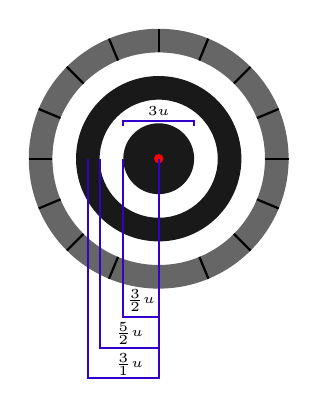
\begin{tikzpicture}[scale=0.3]
\fill[black!90!white] (0,0) circle [radius=1.5];
\fill[black!90!white, even odd rule] (0,0) circle[radius=2.5] circle[radius=3.5];
\fill[black!60!white, even odd rule] (0,0) circle[radius=4.5] circle[radius=5.5];

\foreach \angle in {0, 22.5, 45, 67.590, 90, 112.5, 135, 157.5, 180, 202.5, 225, 247.5, 270, 292.5, 315, 337.5} 
	\draw[thick] (\angle:4.5) -- (\angle:5.5);

\fill[red] (0,0) circle[radius=0.2];

\draw[color=blue!60!violet, thick] (-1.5,1.4) -- ++(0, 0.2) -- ++(1.5, 0) +(0, 0.4)node[black]{\tiny{\(3u\)}}+(0, 0) -- ++(1.5, 0) -- ++(0, -0.2);

\draw[color=blue!60!violet, thick] (0,0) -- (0,-6.7) -- +(-1.5, 0) -- (-1.5,0);
\draw[color=blue!60!violet, thick] (0,0) -- (0,-8) -- +(-2.5, 0) -- (-2.5,0);
\draw[color=blue!60!violet, thick] (0,0) -- (0,-9.3) -- +(-3, 0) -- (-3,0);

\draw (-0.75, -6) node{\tiny{\(\frac{3}{2}u\)}};
\draw (-1.25, -7.4) node{\tiny{\(\frac{5}{2}u\)}};
\draw (-1.25, -8.7) node{\tiny{\(\frac{3}{1}u\)}};
\end{tikzpicture}
  \caption{Größenverhältnisse}
\end{wrapfigure}
Danach gilt es noch zu bestimmen, ob es sich bei dem Kreis um einen Mittelpunkt eines \task{}s handelt, schließlich sollen sonstige Kreise im Bild nicht ausgegeben werden. Hierzu können wir uns die Proportionen eines \task{}s zu nutze machen:

Der Durchmesser ist als \(3u\) definiert, jeder Kreisring und die Zwischenräume haben eine Breite von \(1u\). Daraus folgt, dass wenn man den Mittelpunkt in eine beliebige Richtung um \(3u\) verschiebt, der neue Punkt im mittleren Kreisring liegen muss.

Um nun das Vorhandensein des mittleren Ringes zu überprüfen, nehmen wir vier Punktproben vor. Wir verschieben den Mittelpunkt in alle Himmelsrichtugen um \(u\). Dort vergleichen wir die Länge der entsprechenden linearen Zusammenhangskomponente mit dem Soll \(\1u\). Weitere Punktproben sind prinzipiell möglich, jedoch würden diese die Laufzeit erhöhen. \textbf{Ggfs. weitere Flood-Fill auf Fläche des Kreisringes hinzufügen!}

Die Wahrscheinlichkeit eines Erkennungsfehlers ist nach dem Durchmesservergleich, dem Flächenvergleich und den vier Punktproben sehr gering. Im Beispielbild, dass ich um einen Kreis, der kein \task ist ergänzt habe,liegt die Erkennungsrate bei 100\%.

\pagebreak
\section{Umsetzung}
In meiner Implementierung muss das Delta zwischen der Ist- und Soll-Fläche kleiner als 5\% sein.

Zunächst implementierte ich mithilfe von ImageIO eine Bildeinleseprozedur. Da ImageIO nur RGB-JP(E)Gs, PNGs, BMPs und GIFs einlesen kann, habe ich einen Wrapper für ImageMagick\footnote{\url{http://www.imagemagick.org/}, GPLv3-kompatible freie Lizenz. Enthalten in den Repositories der gängigen Linux-Distributionen, Binarys für weitere Betriebssysteme auf der Entwicklerseite.} geschrieben. Wenn dieser über die entsprechende Checkbox in der GUI zugeschaltet wird, können alle gängigen Bildformate gelesen werden. Nachteil ist eine deutlich längere Einlesezeit. Außerdem muss ImageMagick lokal installiert sein und mit dem Befehl \texttt{convert} aufrufbar sein.\footnote{Getestet unter Arch Linux und Ubuntu Linux 16.10. Weitere Betriebssysteme werden vermutlich auch unterstützt.}

Zunächst überlegte ich mir eine möglichst effiziente Datenstruktur für Grafiken, da die Interaktion über ImageIO mit Bitmaps nicht sonderlich effizient ist. Da für die Erkennung von Kreisen in einer Grafik genaue Informationen über die Farbe eines Bildpunktes nicht relevant sind, kann das Bild beim Einlesevorgang in ein boolesches 2D-Array überführt werden: In diesem Array, das die gleiche Größe wie das eingelesene Bild besitzt, sind die Bildpunkte als True gespeichert, die Teil eines \task{}s sein könnten. In der in Teilaufgabe 1 gegebenen Schwarz-Weiß-Grafik ist diese Einstufung noch simpel: Schwarze Bildpunkte können Teil eines \task{}s sein, sonstige nicht.

Um in diesem Array die Punkte zu bestimmen, deren Kreisradien sich in alle vier Richtungen gleichen, muss zunächst die Länge von aufeinanderfolgenden Streifen aus möglichen \task{}-Feldern ermittelt werden. Diese nenne ich nun lineare Zusammenhängigkeitskomponenten. In seperaten Arrays für horizontale und vertikale Streifen speichere ich für jedes Feld die Länge seiner linearen Zusammenhängigkeitskomponente. Für ein mögliches \task{}-Feld liegt diese für horizontale Zusmmenhängikeitskomponenten bei \(1 \le l \le width\), für vertikale entsprechend bei
\(1 \le l \le height\)
. Bei allen Feldern, die kein Teil einer Zusmmenhängikeitskomponente sind, liegt dieser Wert bei 0. 

Danach kann für jede Koordinate die horizontale und vertikale Zusammenhängigkeitskomponentenlänge verglichen werden. Gleichen sie sich, handelt es sich um einen möglichen Mittelpunkt. Von diesem Punkt aus kann die Soll-Fläche mit der Kreisformel berechnet werden, denn derer Durchmesser des Kreises ist nun mit der Länge einer der beiden Zusammenhängigkeitskomponenten gegeben. Die tatsächliche Länge der Fläche kann mit einer Flood-Fill ermittelt werden.

Schließlich muss noch das Vorhandensein des Kreisringes wie in der Lösungsidee beschrieben verifiziert werden. Auch hier akzeptiert das Programm eine Abweichung im Mittel von 5\%, da durch Anti-Aliasing oder Unschärfen bei der Bildaufnahme Abweichungen vom mathematischen Ideal der Spezifikation zwangsläufig auftreten.
\pagebreak
\section{Beispiele}
Die erkannten Kreismittelpunkte sind mit violetten Kreuzen markiert.
\begin{figure}[!ht]
	\centering	
	\includegraphics[width=\textwidth]{sek1bsp1}
	\caption{Beispielbild d. Aufgabenstellung}
\end{figure}